\chapter{Reinforcement Learning}  
\label{ch:RL}
In diesem Kapitel wird ein erster Einblick in das Reinforcement Learning gegeben, welches ein Teilbereich des Machine Learning ist. Des Weiteren wird genauer auf die verwendeten Netzwerkarchitekturen eingegangen. 

\section{Grundlagen}
\label{sect:RL_Grund}

Machine Learning allgemein ist ein Teilbereich von Artificial Intelligence (AI). Im Zusammenhang mit Daten und Algorithmen wird hierbei versucht, das menschliche Verhalten zu imitieren und zu verbessern \cite{IBM}. Ein typisches Beispiel, das im Zusammenhang mit AI zurzeit sehr präsent ist, ist das autonome Fahren.\\
Das Machine Learning lässt sich in drei Teilbereiche untergliedern:

\begin{itemize}
\item \underline{Supervised Learning} \\
Supervised Learning ist die in Forschungsarbeiten laut \cite{sutton2018reinforcement} meist verwendete Trainingsart im Bereich des Machine Learning. Bei dieser Art erfolgt das Lernen anhand von ausgewählten Beispielen, das von einem erfahrenen und fachkundigen Betreuer beaufsichtigt wird. Für jede Situation aus dieser Beispielmenge gibt es eine korrekte Aktion, die der Agent ausführen soll. Das Ziel ist es, diese Entscheidungen zu verallgemeinern und auf andere Situationen auszuweiten. Diese Form des Lernens ist aber nicht geeignet für das Lösen von interaktiven Problemen \cite{sutton2018reinforcement}. \\


\item \underline{Unsupervised Learning} \\
Beim Unsupervised Learning geht es darum, Strukturen zu finden und diese in verschiedene Cluster einzuordnen. Diese Algorithmen können ohne ein menschliches Eingreifen versteckte Muster entdecken oder Datengruppierungen durchführen. Deshalb ist diese Form des Lernens zum Beispiel ideal für die Bilderkennung \cite{IBM2}.\\

\item \underline{Reinforcement Learning} \\
Beim Reinforcement Learning wird im Gegensatz zu den oben genannten Lernverfahren nicht auf Grundlage von Datensätzen, sondern mittels des so genannten "trial and error" Verfahrens, also durch ausprobieren und scheitern, trainiert. Der Anreiz zum Lernen wird durch Belohnungen erzielt, denn jede mögliche Action des Agenten wird bewertet und anschließend je nachdem belohnt oder bestraft. Es wird also keine Lösung für eine bestimmte Situation vorgegeben, sondern der Agent muss selbst herausfinden, womit er die größte Belohnung erzielen kann. Das Reinforcement Learning bietet eine Vielzahl von Einsatzgebieten, wie zum Beispiel im Gamingbereich oder auch in der Robotik.\\
\end{itemize}

Das Prinzip eines Reinforcement Learning Algorithmus ist in der nachfolgenden Abbildung \ref{RL_Grund} gezeigt.


\begin{figure} [h]
\begin{minipage}[t]{1\textwidth}
\vspace{0pt}
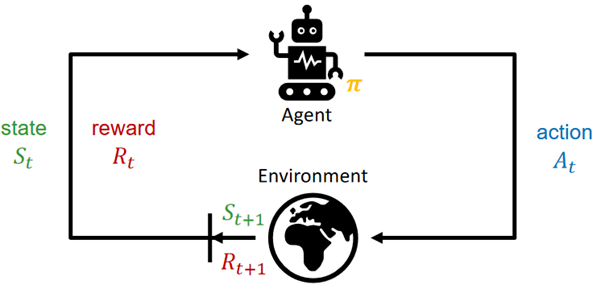
\includegraphics[width=\textwidth]{images/RL_Grundlagen}
 \caption{Übersicht des Reinforcement Learning Prinzips}
\label{RL_Grund}
\end{minipage}
\end{figure}


\begin{itemize}
\item \underline{Agent} \\
Im Agent verbirgt sich der Algorithmus der AI. Er empfängt den aktuellen State und den Reward aus der vorangegangenen Action und entscheidet unter Berücksichtigung der Policy, welche Action nun die beste Lösung im Verlauf der Episode bringen wird. Das Ziel des Agenten ist, einen möglichst großen Reward zu erzielen. Bei diesem Projekt ist der Agent der Pusher des Roboters.
\item \underline{Environment} \\
Das Environment zeigt die Gegebenheiten, auf deren Grundlage das Problem gelöst werden soll. Es gibt dem Agenten den Reward aus seiner vorangegangen Action zurück. In diesem Projekt ist das Environment ein Airhockeytisch. 
\item \underline{Action} \\
Eine Action wird vom Agenten zum Environment geschickt. Dort wird anschließend diese dann ausgeführt. In diesem Projekt bilden die neun Richtungsmöglichkeiten die Menge aller möglichen Actions.
\\item \underline{State} \\
Ein State ist der aktuelle Zustand des Spiels, nachdem eine Action im Environment durchgeführt wurde. Der State in diesem Projekt wird über die Kamera aufgenommen und weitergegeben.
\item \underline{Reward} \\
Mithilfe von Rewards wird der Agenten trainiert. Zu jedem Zeitpunkt gibt das Environment an den Agenten diesen Reward zurück. Ziel des Agenten ist es, den größtmöglichen Reward am Episodenende zu erreichen. Die Rewards in diesem Projekt werden genauer im Kapitel \ref{sect:rewards_params} erläutert.
\item \underline{Policy $\pi$} \\
Die Policy  bestimmt das Verhalten des Agenten. Es nimmt den aktuellen Zustand des Environments auf und wählt die darauffolgende Action aus. 
\item \underline{Episode} \\
Eine Episode ist ein vorgeschriebener Zeitraum, nach dem das Environment wieder in den Ursprungszustand zurückgesetzt wird. Sie können entweder nach einer bestimmten Zeit terminiert werden oder aber abhängig von einem State beendet werden. Bei diesem Projekt zum Beispiel endet eine Episode unter anderem, wenn ein Tor erzielt wurde. Danach wird das Environment wieder auf die Ausgangslage zurückversetzt und es kann weiter trainiert werden. Der Agent behält jedoch seinen Trainingsfortschritt aus den vorangegangenen Episoden bei.
\end{itemize}


\begin{figure} [h]
\begin{minipage}[t]{1\textwidth}
\vspace{0pt}
Die Abfolge von State (S), Reward (R) und Action (A) ist zu Beginn wie folgt festgelegt (Der Index gibt an, um welchen Zeitschritt es sich handelt): $S_{0}$, $A_{0}$, $R_{1}$, $S_{1}$, $A_{1}$, $R_{2}$, $S_{2}$, $A_{2}$, $R_{3}$, ...   

Zu Beginn beeinflusst das Verhalten des Agents nur der aktuelle State $S_{0}$. Unter Berücksichtigung der Policy führt der Agent eine Action $A_{0}$ zum State $S_{0}$ durch. Das Environment führt nun eine Beurteilung des daraus resultierenden neuen State $S_{1}$ durch und gibt dem Agent dementsprechend einen neuen Reward $R_{1}$ zurück. Diese Schleife wird solange durchgegangen, bis das Ende der Episode erreicht wurde.

\end{minipage}
\end{figure}
\clearpage

\section{Reinforcement Learning Algorithmus}
\label{sect:RL_Algo}
Die Grundlage des Reinforcement Learning ist die einfache mathematische Beschreibung des Problems als Markow Decision Process. Hierbei werden nur der State und die Action, welche unmittelbar zuvor aufgetreten sind, berücksichtigt.
Ein Reinforcement Algorithmus kann in zwei Bereiche aufgeteilt werden \cite{CarnegieMellonUniversity}: 
\begin{itemize}
\item \underline{Model-Based} \\
Der Hauptbestandteil der Model-Based Methode ist die Planung einer Lösung des Problems. Der Agent analysiert das Environment, versucht es zu verstehen und dementsprechend eine Action auszuwählen.
\item \underline{Model-Free} \\
Bei der Model-Free Methode wird nicht das Modell des Environments genau analysiert und erlernt, sondern das Lernen erfolgt nur durch Probieren.
\end{itemize}
Des Weiteren können die Methoden dahingehend unterschieden werden, ob sie On-Policy oder Off-Policy sind. Der Unterschied ist, dass bei Off-Policy nur der nächste State berücksichtigt wird, während bei On-Policy auch noch die aktuelle Action in den Entscheidungsprozess mit einfließt \cite{aracom}. Des Weiteren ist es bei Off-Policy Algorithmen möglich, aus den Erfahrungen, die in der Vergangenheit gesammelt wurden, zu lernen \cite{ppo_git}. \\

Es existiert eine Vielzahl an Algorithmen. Jeden einzeln zu beschreiben würde den Rahmen dieser Arbeit sprengen. Deshalb werden im Folgenden nur zwei Beispiele gegeben. Da später das Training mit dem Proximal Policy Optimization (PPO) und dem Soft Actor-Critic (SAC) durchgeführt wird (vgl. Kapitel \ref{subsect:netzwahl_ergs}), werden diese beiden Netzwerke nun genauer erläutert. 

\subsection{Proximal Policy Optimization (PPO)}
\label{subsect:ppo}
Da die Algorithmen der Reinforcement Learning Methoden schwer zu handhaben sind und sehr aufwendig in der Abstimmung sind, wurde der PPO Algorithmus entwickelt. Das Prinzip hierbei ist, möglichst ein Gleichgewicht zwischen einer einfachen Implementierung, einer einfachen Abstimmung und der Komplexität der Beispiele zu finden. Dazu wird in jedem Schritt die Kostenfunktion minimiert, jedoch darf die Abweichung zur bisherigen Policy nur gering sein \cite{ppo}.
Gemäß \cite{ppo_git} wird bei der Verwendung des ML-Agents Toolkit in Unity (vgl. Kapitel \ref{ch:Simulationsumgebung}) als Grundeinstellung dieser Algorithmus ausgewählt. Die Erfahrung hat gezeigt, dass dieser einen großen Einsatzbereich hat und stabiler ist als viele andere.

\subsection{Soft Actor-Critic (SAC)}
\label{subsect:sac}
Im Unterschied zum PPO Algorithmus wird beim SAC auf die Erfahrungen aus den vorangegangenen Zeitpunkten zurückgegriffen und die Erkenntnisse daraus zufällig wieder herangezogen. Der Vorteil gegenüber dem PPO ist dadurch, dass weniger Stichproben gebraucht werden. Ein SAC bietet sich dann an, wenn man ein schweres und langsames Environment hat \cite{ppo_git}.



